%%%%%%%%%%%%%%%%%%%% author.tex %%%%%%%%%%%%%%%%%%%%%%%%%%%%%%%%%%%
%
% template for Encyclopedia articles
%
%%%%%%%%%%%%%%%% Springer %%%%%%%%%%%%%%%%%%%%%%%%%%%%%%%%%%


% RECOMMENDED %%%%%%%%%%%%%%%%%%%%%%%%%%%%%%%%%%%%%%%%%%%%%%%%%%%
%\documentclass[graybox, natbib, nosecnum, twocolumn]{svmult}
\documentclass{svjour3}
\usepackage[english]{babel}
\usepackage[utf8x]{inputenc}
\usepackage[T1]{fontenc}

%% Sets page size and margins
\usepackage[a4paper,top=3cm,bottom=2cm,left=3cm,right=3cm,marginparwidth=1.75cm]{geometry}

%% Useful packages
\usepackage{amsmath}
\usepackage{graphicx}
\usepackage[colorinlistoftodos]{todonotes}
\usepackage[colorlinks=true, allcolors=blue]{hyperref}

%%%%%%%%%%%%%%%%%%%%%%%%%%%%%%%%%%%%%%%%%%%%%%%%%%%%%%%%%%%%%%%%%%%%%%%%%%%%%%%%%%%%%%%%%

\begin{document}

\title{Historical Graph Data Management}
% Use \titlerunning{Short Title} for an abbreviated version of
% your contribution title if the original one is too long
\author{Udayan Khurana and Amol Deshpande}
% Use \authorrunning{Short Title} for an abbreviated version of
% your contribution title if the original one is too long
\institute{Udayan Khurana
		\at IBM Research AI, TJ Watson Research Center, Yorktown Heights New York NY, USA \\\email{ukhurana@us.ibm.com}
		\and
		Amol Deshpande
		\at Computer Science Department, University of Maryland, College Park MD, USA \\\email{amol@cs.umd.edu}
		}
%
% Use the package "url.sty" to avoid
% problems with special characters
% used in your e-mail or web address
%
\maketitle

\begin{abstract}
%Your abstract.
%\end{abstract}

%\section{Introduction}
Real world graphs evolve over time, with continuous addition and removal of vertices and edges, as well as frequent change in their attributes. Some examples of such graphs are phone-call graphs generated by telecommunication service providers, message graphs from social networking sites, and mention-activity graphs formed by Twitter users mentioning one another in their tweets.
For decades, the work in graph analytics was restricted to a static perspective of the graph. Analysis such as finding important (central) entities in a network, groups (clusters) of similar entities, observing graph density, diameter and several other attributes have been well studied in the context of static graph snapshots. 
In recent years, however, we have witnessed an increasing abundance of timestamped observational data describing
various types of temporal information networks, including social networks, biological networks,
citation networks, financial transaction networks, communication networks, to
name a few. This has fueled an interest in performing richer analysis of graphs, along a temporal dimension. Analysis of history of a graph presents fascinating insights into the underlying phenomena that produced the graph. 
However, the traditional network data management systems are inadequate for such analyses. We present a summary of recent advances in the field of historical graph data management . They involve, compact storage of large graph histories, efficient retrieval of temporal subgraphs, and effective interfaces for expressing historical graph queries are essential for enabling temporal graph analytics.  
\end{abstract}

\section{Overview}
In recent years, many works have focused on designing analytical models that capture how a network evolves, with a primary focus on
social networks and the Web (see, e.g., ~\cite{LeskovecKF07,Kumar:2006:SEO:1150402.1150476}).
There is also much work on understanding how communities evolve, identifying key individuals,
and locating hidden groups in dynamic networks. Berger-Wolf et
al.~\cite{Berger-Wolf2006,tantipathananandh2007framework},  
%present a framework that focuses on identifying communities and understanding how they change over time.
Tang et al.~\cite{tang2008community} and Greene et al.~\cite{Greene2010} 
address the problem of community evolution in
dynamic networks.
McCulloh and Carley~\cite{McCulloh2008} present techniques for social change detection.
Asur et al.~\cite{Asur2009} present a framework for characterizing the complex behavioral patterns
of individuals and communities over time. %Biologists share on predicting historical events leading to a 
%known biological network (e.g.,~\cite{10.1371/journal.pcbi.1001119})
Biologists are interested in discovering historical events leading to a 
known state of a Biological network (e.g.,~\cite{10.1371/journal.pcbi.1001119}).
Evolution of shortest paths in dynamic
graphs has been studied by Huo et al.~\cite{huo2014efficient}, Ren et al.~\cite{RenEvolvGraph11},
and Xuan et al.~\cite{xuan2003computing}. Change in page rank with evolving graphs~\cite{desikan2005incremental,bahmani2010fast}, and
the study of change in centrality of vertices, path lengths of vertex pairs,
etc.~\cite{pan2011path}, also lie under the larger umbrella of temporal graph analysis.
Barrat et al.~\cite{barrat2008dynamical}, provide a good reference for studying several
dynamic processes modeled over graphs. Holme et al.~\cite{holme2012temporal} provide a description of several networks from different domains that 
are temporal or dynamic in nature.


The purpose of this chapter is to highlight the recent advancements in graph data management system that can efficiently and scalably
support these types of dynamic network analysis tasks over large volumes of data. The static graph data management systems are insufficient in supporting the analytical tasks described above, primarily due to a lack of understanding of the {\em change} or {\em difference} in graphs. The temporal graph analyses solutions based upon such systems become too expensive in storage costs, memory requirements, and often unfriendly or infeasible for an analyst to express in the first place. 
As per the terminology of temporal relational databases, this discussion considers \textbf{valid time} (against \textbf{transaction time}) as the underlying temporal dimension for historical analyses. Valid time denotes the time
period during which a fact is true with respect to the real world. Transaction time is the time
when a fact is stored in the database. 
It is worth noting that there is a related but orthogonal body of work which we do not touch in this chapter. It deals with the need to do {\em real-time analytics on the streaming data} as it is being generated; here the scope of the analysis typically only includes the latest snapshot or the snapshots from a recent window. The key challenge here is to be able to deal with the high rate at which the data is often generated.


\begin{figure}
\centering
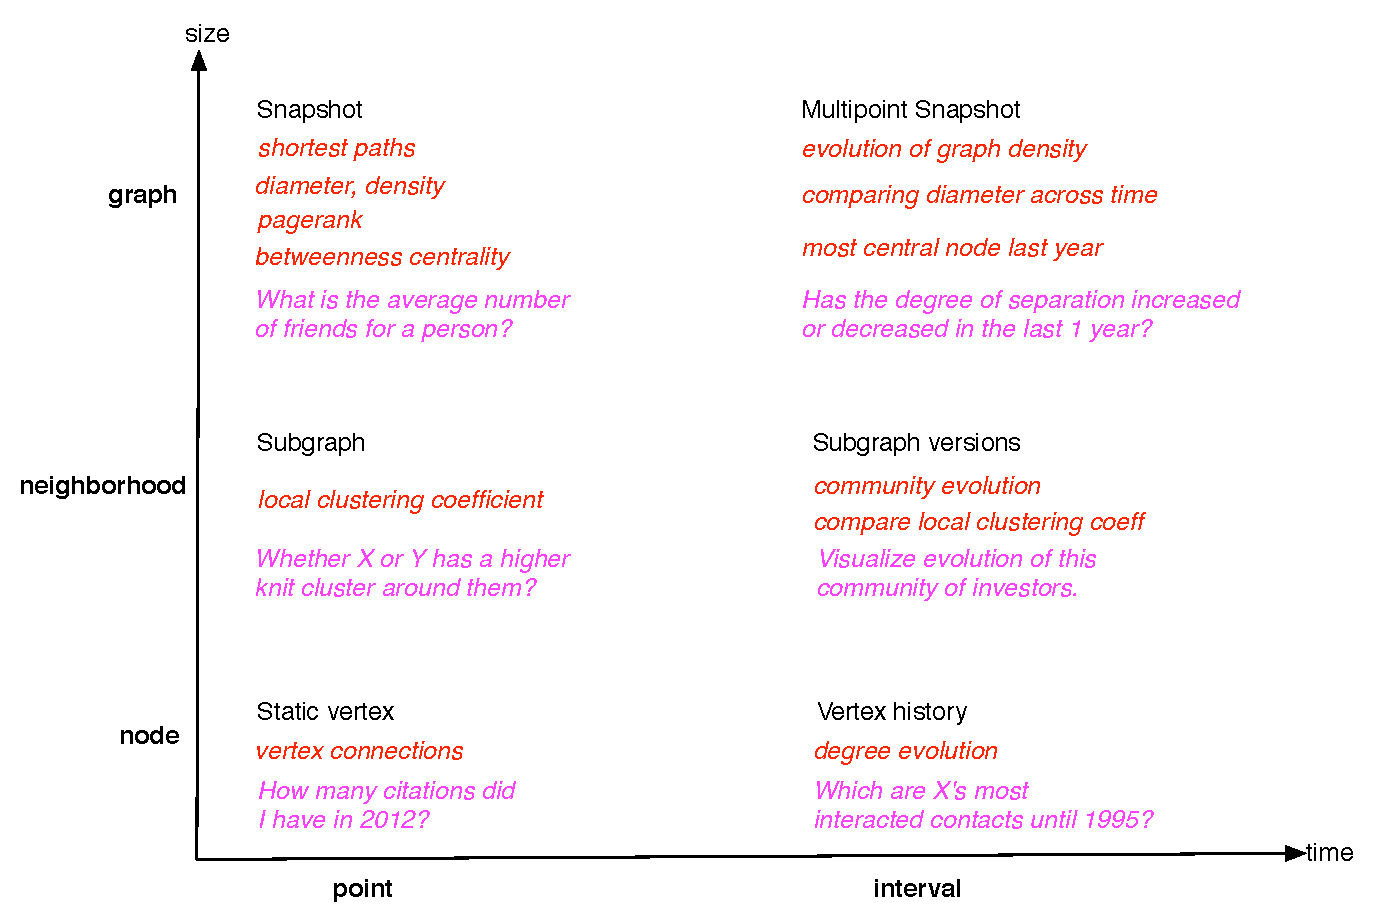
\includegraphics [width=0.85\textwidth]{entity-time.pdf}
\caption{A temporal graph can be represented across two different dimensions - time
and entity. The chart lists retrieval tasks (black), graph operations (red), example queries
(magenta) at different granularities of time and entity size.}
\label{fig:et}
\end{figure}

%Main Text

TODO:
Categorize different types/rates of change. Refer to Figure 1 on how different changes w.r.t. scope of the graph and timespan correspond to different analytical tasks and also different data management 
Ahn et al.~\cite{ahn2014task} present an exhaustive taxonomy of temporal tasks. 


The frequent change of a temporal graph poses a significant challenge to algorithm design, because the overwhelming majority of graph algorithms assume static graph structures. One would have to design special algorithms for each application to accommodate the dynamic aspects of graphs. To support general-purpose computations, most of the temporal graph systems adopt a strategy to separate graph updates from graph computation. More specifically, although updates are continually applied to a temporal graph, graph computation is only performed on a sequence of successive \emph{static} views of the temporal graph. For simplicity, most systems adopt a \emph{discretized-time} approach, so that time domain is set of natural numbers, i.e., $t\in \mathcal{N}$. 

The separation of graph update and graph computation not only allows existing algorithms designed for static graphs to be used for analyzing temporal graphs, but also enables the same familiar computation interface in existing static graph processing systems to be used for temporal graphs. In fact, TIDE employs the message passing-based vertex-centric programming model like in Pregel~\cite{pregel} for analyzing dynamic graphs, while Kineograph and Chronos use the vertex-centric scatter-gather model (like the GAS model of GraphLab~\cite{graphlab}) in either a pull mode or a push mode. In addition, Chronos can also support the edge-centric model proposed in X-Stream~\cite{xstream}.


Broadly speaking the focus of this work is on providing the ability to analyze and to reason over the entire history of 
the changes to a graph. There are many different types of analyses that may be of interest. 
For example, an analyst may wish to study the evolution of well-studied static graph properties such
as centrality measures, density, conductance, etc., over time. Another approach is through the search and 
discovery of temporal patterns, where the events that constitute the pattern are spread out over time. 
Comparative analysis, such as juxtaposition of a statistic over time, or perhaps, computing 
aggregates such as \textit{max} or \textit{mean} over time, possibly gives another style of knowledge discovery 
into temporal graphs. Most of all, a primitive notion of just being able to access past states of the graphs 
and performing simple static graph analytics, empowers a data scientist with the capacity to 
perform analysis in arbitrary and unconventional patterns.

Supporting such a diverse set of temporal analytics and querying over large volumes of historical graph data 
requires addressing several data management challenges. Specifically, we need techniques for storing
the historical information in a compact manner, while allowing a user to retrieve graph snapshots as of any
time point in the past or the evolution history of a specific node or a specific neighborhood. Further the
data must be stored and queried in a distributed fashion to handle the increasing scale of the data.
We must also develop an expressive, high-level, easy-to-use programming framework that will allow users to 
specify complex temporal graph analysis tasks, while ensuring that the specified tasks can be executed efficiently 
in a data-parallel fashion across a cluster.




\section{Storage and Retrieval}

Storage of large temporal graphs is challenging and requires careful design. A straightforward use of static graph datastore can lead to a potential explosion in storage requirements, and/or incur high latency times for retrieving sub-graphs, or timeslices. The most straightforward being the storage of 
In this section, we present the most recognized approaches for efficient storage and retrieval of historical graphs.

Salzberg and Tsotras~\cite{Salzberg1999} present a comprehensive
survey of temporal data indexing techinques, and discuss two extreme approaches 
to supporting snapshot retrieval queries, referred to as the \textit{Copy} and \textit{Log} approaches. While the copy approach relies on storing new copies of a snapshot upon every point of change in the database, the log approach relies on storing everything through changes. Their hybrid is often referred to as the \textit{Copy+Log} approach.%We omit a detailed discussion of the work on temporal databases, and refer the interested reader to a representative set of references~\cite{Bolour92,DBLP:conf/sigmod/SnodgrassA85,Ozsoyoglu1995,Tansel1993,date2002temporal,tsql2,Salzberg1999}. 
Other data structures, such as Interval Trees~\cite{Arge1996} and Segment trees~\cite{Blankenagel1994} can also be used for storing temporal information. Temporal aggregation in scientific array databases~\cite{soroush2013time} and time-series indexing~\cite{niennattrakul2010exact}, ~\cite{camerra2013beyond}, ~\cite{wang2013experimental} are other related topics of interest, but the challenges there are significantly different.

TODO: all other temporal db references go here


\subsection{Deltas-based Encodings}
The original DeltaGraph~\cite{khurana2013efficient} system only supported retrieval of individual snapshots of the historical graph as of specific time instances. Here we instead discuss the extension of that work~\cite{khurana2016storing} that allows retrieval of different temporal graph primitives including neighborhood versions, node histories, and graph snapshots, and that features a temporal graph analysis framework built on top of Apache Spark. 

\vspace{2mm}
\noindent{\bf Temporal Graph Index.} DeltaGraph organizes the historical graph data in a hierarchical data structure, whose lowest level corresponds
to the snapshots of the network over time, and whose interior nodes correspond to graphs constructed by ``combining''
the lower level snapshots in some fashion; the interior nodes are typically not valid snapshots as of any specific time point. Neither the lowest-level
graph snapshots nor the graphs corresponding to the interior nodes are actually stored explicitly. Instead, for each edge, a {\em delta}, i.e., the
difference between the two graphs corresponding to its endpoints, is computed, and these deltas are explicitly stored. In addition, the graph
corresponding to the root is explicitly stored. Given those, any specific snapshot can be constructed by traversing any
path from the root to the node corresponding to the snapshot in the index, and by appropriately combining the information present in the deltas.
Use of different ``combining'' functions leads to a different point in the performance-storage trade-off, with {\em intersection} being the most
natural such function.  This index structure especially shines with multi-snapshot retrieval queries which are expected to be common in temporal 
analysis, as it can share the computation and retrieval of deltas across the multiple snapshots.
The index structure is also {\bf extensible}, providing a user the opportunity to define additional 
indexes to be created and maintained in order to efficiently execute specific queries (e.g., subgraph pattern matching, reachability, etc.)
    over the historical graph data.

To facilitate distributed storage and parallel retrieval, the deltas themselves are partitioned horizontally by nodes and vertically by attributes 
of the nodes, and these partitions are stored in a key-value store (specifically, Apache Cassandra). This allows efficient retrieval of not only
entire snapshots, but also of individual neighborhoods or temporal histories of individual neighborhoods.


\subsection{Indexing based on Time Locality}
Chronos~\cite{han2014chronos} targets time-range graph analytics, requiring computation on the sequence of static snapshots of a temporal graph within a time range. An example is analyzing the change of each vertex's PageRank for a given time range. Obviously, the most straightforward approach of applying computation on each snapshot separately is too expensive. Chronos achieves efficiency by exploiting locality of temporal graphs.

\vspace{2mm}


\noindent{\bf On-Disk Graph Layout.} Chronos also leverages the time locality to store temporal graphs on disk in a compact way. The layout is organized in snapshot groups. A snapshot group $G_{t_1,t_2}$ contains the state of $G$ in the time range $[t_1,t_2]$, by including a checkpoint of the snapshot of $G$ at $t_1$ followed by all the updates made till $t_2$. The snapshot group is physically stored as edge files and vertex files in time-locality fashion. For example, an edge file begins with an index to each vertex in the snapshot group, followed by segments of vertex data. The segment of a vertex, in turn, first contains a set of edges associated with the vertex at the start time of the snapshot group, followed by all the edge updates to the vertex. A link structure is further introduced to link edge updates related to the same vertex/edge, so that the state of a vertex/edge at a given time $t$ can be efficiently constructed.

\subsection{Multiversion Arrays etc.}
So far, we have only reviewed distributed temporal-graph systems. There also exist some single-machine systems that support graph analytics on temporal graphs. In this subsection, we introduce a single-machine system called LLAMA~\cite{macko2015llama} for storing and analyzing evolving graphs. LLAMA aims at applications that receive a steady stream of graph updates, but need to perform various whole-graph analysis on consistent views. It is worth mentioning that there also exist some single-machine temporal-graph systems for specific types of graph queries. For example, EAGr~\cite{eagr} is an in-memory system for continuously answering ego-centric aggregate queries on a temporal graph, where a query computes an aggregate in the neighborhood of a vertex over a recent time window.

LLAMA is a single machine system that stores and incrementally updates an evolving graph in multi-version representation, and it supports both in-memory and out-of-core graph analysis on graph snapshots. LLAMA provides a general-purpose programming model, though vertex-centric or edge-centric computations can be implemented on top of it.

In LLAMA, an evolving graph is modeled as a time series of graph snapshots, where each batch of incremental updates produces a new graph snapshot. The graph storage is read-optimized, while the update buffer is write-optimized.

The most important contribution of LLAMA is that, it augments the compact read-only CSR representation to support mutability and persistence. Specifically, a graph is represented by a single vertex table, and multiple edge tables, one per snapshot. The vertex table is organized as a large multi-versioned array (LAMA) that uses a software copy-on-write technique for snapshotting, and the record of each vertex $v$ in the vertex table maintains the necessary information to track $v$'s adjacency list from the edge tables across snapshots.

We now review the LAMA data structure for representing the vertex table. Specifically, the array of records is partitioned into equal-sized data pages, and an indirection array is constructed that contains pointers to the data pages. The indirection array fits in L3 cache. To create a new snapshot, the indirection array is copied, with those references to out-dated pages replaced by those to the newly modified pages. Thus, we do not need to copy unmodified pages across snapshots. LAMA stores 16 consecutive snapshots of the vertex table in each file, so that disk space can be easily reclaimed from deleted snapshots.

The edge table for a snapshot $i$ is organized as a fixed-length array that stores adjacency list fragments consecutively, where each adjacency list fragment contains the edges of a vertex added in snapshot~$i$. An adjacency list fragment of vertex $v$ also stores a continuation record, which points to the next fragment for $v$, or {\em null} if there are no more edges. To support edge deletion, each edge table may maintain a deletion vector, which is an array that encodes in which snapshot an edge was deleted.

Properties on vertices and edges may change and should also support snapshotting. Like the vertex table, each type of property is also stored with a LAMA. Different types of properties are stored in separate LAMAs, so that a job may only load the needed property (or properties) for graph analysis.

LLAMA buffers incoming updates in a write-optimized lookup table, which stores the newly-added and deleted edges for each vertex. The buffered updates are only written into a new snapshot, and a graph analytics query only runs on the read-optimized graph storage without checking the table of buffered updates.





\section{Historical Graph Analytics}

\subsection{Runtime Environments}

\noindent{\bf In-Memory Graph Layouts.} Talk about overlaid graph layout - GraphPool, Chronos (LABS).  

\noindent{\bf Incremental Computation.} goes here.

\noindent{\bf Parallelization.} TGAF - no overlaying but that is useful for Spark-based parallelization. Talk about RDD based temporal graph abstraction
Llama parallelization. Potential of parallelization based on multi time-point computation.


TODO: Use the following material.

GraphPool, Chronos, TGAF Spark, etc. Mention the data structures, parallelization, temporal compression.

\vspace{2mm}
\noindent{\bf Temporal Graph Analysis Framework.} The second, somewhat orthogonal, component of this system is a Apache Spark-based analysis
framework to specify temporal graph analysis tasks. This analysis framework is based on an abstraction of a \textit{set of nodes 
(or subgraphs) evolving over time}. Several operations are supported on top of this abstraction, including selection, timeslicing, and
temporal {\em map} and {\em reduce} operations. The library is implemented in Python and Java, is built on top of Apache Spark, and also provides
integration with GraphX for executing graph algorithms supported by that system.



\noindent{\bf In-Memory Graph Layout.} There are two kinds of locality for temporal graphs that can be exploited for efficient data layout: \emph{time} locality, where states of a vertex (or an edge) in consecutive snapshots are stored together; and \emph{structure} locality, where states of neighboring vertices in the same snapshot are laid out close to each other. Due to the complex structure of a graph, structure locality is very hard to achieve. Chronos thus favors time locality for graph layout. The selected snapshots for a temporal graph in a time range are stored together in a vertex data array and an edge array. In the vertex data array, data is grouped by the vertices. The data of a vertex in consecutive snapshots are placed together. In the edge array, all the edges are grouped by the source vertices. Inside each group, every edge stores the target vertex ID and a bitmap indicating the snapshots that contain the edge. 
%Although storing all the snapshots in this aggregate form has some similarity to the aggregate graph concept in TIDE, they are used in different context. TIDE stores sample graphs at the same time point together, whereas Chronos stores snapshots in different time points together.

\vspace{2mm}

\noindent{\bf Scheduling of Graph Computation.} To leverage the time-locality graph layout, Chronos employs the locality-aware batch scheduling (LABS) of graph computation. More specifically, LABS batches the processing of a vertex across all the snapshots, as well as the information propagation to a neighboring vertex for all the snapshots. %This batching is similar to the bulk execution model in TIDE, but again TIDE uses it for different sample graphs at the same time point instead of snapshots at different time points. 
In~\cite{han2014chronos}, the authors show that with a simple partition-by-vertex strategy, LABS significantly improves the performance of graph computation in a multi-core parallel setting.

\vspace{2mm}

\noindent{\bf Incremental Computation.} Since Chronos targets at time-range graph analysis, it benefits more from incremental computation. Besides the incremental approach discussed at the end of Section~\ref{ssec:dynamicOverview}, Chronos proposes two enhancements. First, if the target time-range contains a sequence of $N$ snapshots $S_0$ to $S_{N-1}$, it first computes on $S_0$, and then uses the final states of $S_0$ as the initial states for $S_1$ to $S_{N-1}$, and computes the remaining $N-1$ snapshots in one batch using LABS. In the second enhancement, Chronos pre-computes the intersection (or the union) of the $N$ snapshots, applies graph computation on the intersection (or union) graph first, and then uses the final states of this computation as the initial states for all the snapshots and computes all the snapshots in a batch. The second enhancement allows incremental algorithms designed for edge-insertion only to work with temporal graphs with edge deletion.

\vspace{2mm}



\subsection{Interfaces}
Talk about programmatic interfaces first Temporal graph algebra - TGAF etc., Julia Stoyanovich's papers. 

In second paragraph, talk about visual analytics.

Visualization is a an effective tool in exploring and analyzing a temporal graph. Following is a rather brief and non-exhaustive list of techniques and tools that provide such capabilities. 
Erten et al.~\cite{erten2004exploring} present visual analysis for an evolving dataset in computing literature through properties like diameter, connected components, collaborators, co-authors, topic trends over time.
Using visualization of different snapshots, Toyoda et al.~\cite{toyoda2005system} study events like appearance of pages, relationship between different pages for a historical dataset of Web archive.
More such examples can be found in a survey by Kerracher et al.~\cite{kerracher2015task}. Different visualization techniques are useful in the process of gaining insights into the temporal nature of graphs. For instance, NetEvViz~\cite{khurana2011visual} extends NodeXL, to study evolving networks. It uses an edge color coding scheme for comparative study of network growth. Ahn et al.~\cite{ahn2011temporal} focus on different states of graph components in order to visualize temporal dynamics of a social network.
Alternate representations to node-link diagrams have been proposed in order to study temporal nature of social networks, such as TimeMatrix~\cite{yi2010timematrix} that uses a matrix based visualization to better capture temporal aggregations and overlays. A temporal evolution analysis technique based on capturing visual consistency across snapshots can be seen in the work of Xu et al.~\cite{xu2011visualizing}.
A survey by Beck et al.~\cite{beck2014state} lists several other approaches for visual analysis of dynamic graphs. 



\bibliographystyle{alpha}
\bibliography{sample} %for bibtex-example

%For non-Bibtex users:
%\begin{thebibliography}{99}
%\bibitem[Aron 2001]{Aron01} Aron J, Blass B (2001) The future of modern genomics. Blackwell, London
%\bibitem[Brown 2001]{Brown01} Brown B, Aaron M (2001) The politics of nature. In: Smith J (ed) The rise of modern genomics, 3rd edn. Wiley, New York, p 234 -295 
%\bibitem[Smith 1999] {Smith99} Smith J, Jones M Jr, Houghton L et al (1999) Future of health insurance. N Engl J Med 965:325 -329  
%\bibitem[South 1999]{South99} South M (1999) The future of genomics. In: Williams H (ed) Proceedings of the genomic researchers, Boston, 1999
%\end{thebibliography}

\end{document}

